\chapter{The Pressure Signature of Aeroacoustic Sources}
Reference Ani's work here???

\section{Preprocessing: Filtering the Actuator Self-Noise}
Analysis of the near-field response of the forced jet is not immediately straightforward due to acoustic contamination from the actuators themselves [Kearney-fisher]. 
LAFPAs operate on a joule heating principle - the breakdown of the air between the electrodes and the ensuing flow of current results in intense heating of the air. This rapid, localized thermal perturbation produces a compression wave, which excites the shear layer. 
However, this compression wave is still evident as it travels through the near field. 
Multiple compression waves can clearly be seen in \fig{fig:self-noise}, in which a subsonic rectangular jet is being excited at 20 kHz by four LAFPAs on its lower edge. 
\begin{figure}
	\centering
	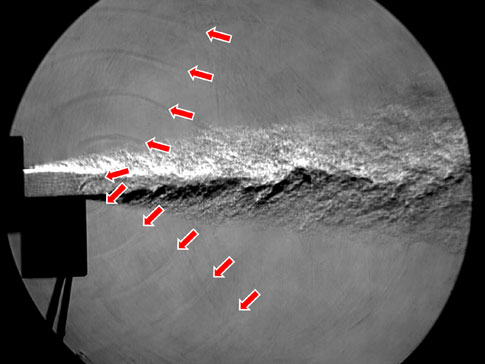
\includegraphics{Figures/Samimy2010JFM.jpg}
	\caption{Schlieren image highlighting LAFPA compression waves. Reprinted from Samimy 2010 JFM.}
	\label{fig:self-noise}
\end{figure}

Obviously, this is an undesirable effect, as this actuator self-noise may in some cases obscure the hydrodynamic and acoustic response of the jet.
So, in the present work the near-field pressure signals have been preprocessed using a continuous-wavelet-based filtering algorithm, which has been specifically designed to remove the actuator self-noise while leaving the signature of the jet response unaltered. 
An example of this filtering can be found in \fig{fig:preprocessing:wavelet_filter}, where the raw and preprocessed signals have been plotted for $St_{DF} = 0.02$ at $x/D = 1$, $r/D = 1.20$. 
To aid in visualization, the results for multiple excitation periods has been phase-averaged to produce these waveforms. 
As the actuator self-noise is localized in both time and frequency and can be well predicted, a smoothing algorithm in the wavelet domain was found to be the most effective method for removing the undesirable noise while leaving the response of the jet intact. 
A fourth-order Paul wavelet is employed, due to the similarity of its imaginary component to the phase-averaged response of the jet. 
As a result, the energy of the response of the jet is well defined in the wavelet domain, with the actuator self-noise existing as high-frequency, temporally-localized oscillations superimposed on the field. 
After smoothing in the wavelet domain to remove these oscillations, the signal is transformed back into the physical domain where it undergoes another smoothing operation in order to remove small amplitude, high frequency oscillations which may be introduced by the wavelet-smoothing. 
For consistency hereafter, all results examined within this work have been computed from the filtered, rather than the raw, signals.
\begin{figure}
	\centering
	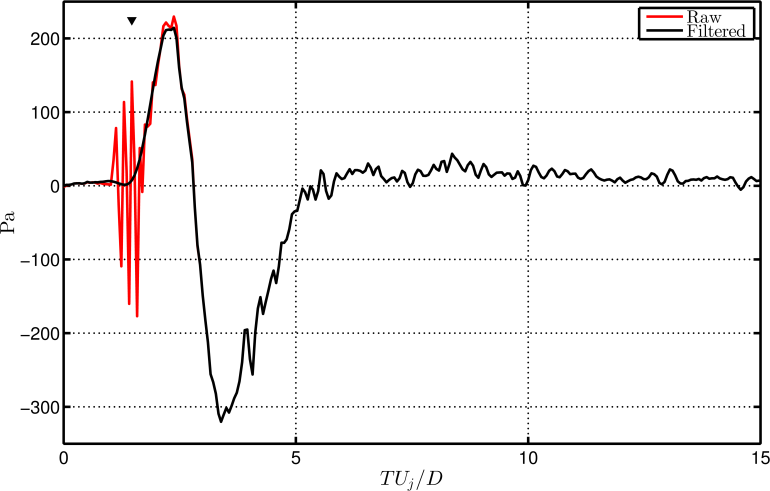
\includegraphics{Figures/NearField_Preprocessing_Filtering.png}
	\caption{Raw and preprocessed near-field pressure.}
	\label{fig:preprocessing:wavelet_filter}
\end{figure} 

\section{Far-field Response}
\section{Acoustic/Hydrodynamic Decomposition}
Much of the difficulty in identifying the aeroacoustic source terms revolves around the dissimilar range of scales and fluctuation intensities of the turbulent eddies in the shear layer and the resulting radiated noise. 
Outside the jet shear layer, in the irrotational near-field of the jet, strong hydrodynamic pressure fluctuations associated directly with the passage of coherent structures in the shear layer and their resultant weak acoustic radiation coexist [Arndt]. 
Beyond this, in the acoustic far-field, the hydrodynamic signature of the coherent structures is nonexistent owing to their strong exponential decay with radial distance.
It is in the irrotational near-field that much work has focused, in order to improve the aeroacoustic community’s understanding of the link between shear layer turbulence and far-field acoustic radiation. 

Owing to the presence of strong hydrodynamic fluctuations dominating the irrotational pressure field near the noise source regions, identification of pure acoustic waves and their corresponding source events is problematic.
A decomposition of the pressure field into its constitutive hydrodynamic and acoustic components is therefore required. 
By identification and prediction of coherence nulls in the near field, Coiffet \etal [cite] showed that the full irrotational near-field consistent primarily as a linear superposition of its hydrodynamic and acoustic components, which lead subsequent researchers to propose linear filters to extract the individual components from the near-field pressure, with varying degrees of success. 

In a subsonic jet (or a transonic jet) in which the large-scale structures are convecting subsonically with respect to the ambient speed of sound, a demarcation of the hydrodynamic and acoustic energy fields can be observed with phase velocity.
An illustration of this can be found in \fig{fig:phase_velocity_map}, where the power spectral density of the irrotational near-field pressure for a single microphone array position has been plotted as a function of normalized frequency and (axial) wavenumber.
The sonic velocity has been identified with a dashed line; energies lying above this line correspond to supersonically traveling waves (and hence, acoustic energy) whereas energies below this line correspond to subsonically convecting waves (hydrodynamic energy).
Note that at high wavenumber and frequencies, two distinct energy lobes become readily apparent.

This phase-velocity separation is the basis for the decomposition method of Tinney \& Jordan [cite], which used a Fourier-based wavenumber-frequency filter in a cold, subsonic jet to separate the near-field pressure into supersonically- and subsonically-convecting waves. 
Grizzi \& Camussi [cite] took a slightly different approach, which utilized a discrete wavelet transform at individual spatial locations in order to decompose the fields based on an energy cutoff. 
The energy threshold was set iteratively, using analysis of two-point correlations of the acoustic and hydrodynamic components between two microphones, in order to ensure that realistic phase-velocities for the components were met. 
The Empirical Mode Decomposition (EMD) based method of Kuo \etal [cite] dispensed with explicit concerns with the phase velocity of the pressure components and instead used the critical frequency, as defined by Arndt \etal [cite], which demarcates the energy dominance of the acoustic and hydrodynamic components in the near-field spectra.
[Include recent Yonglu paper?]
\begin{figure}
	\centering
	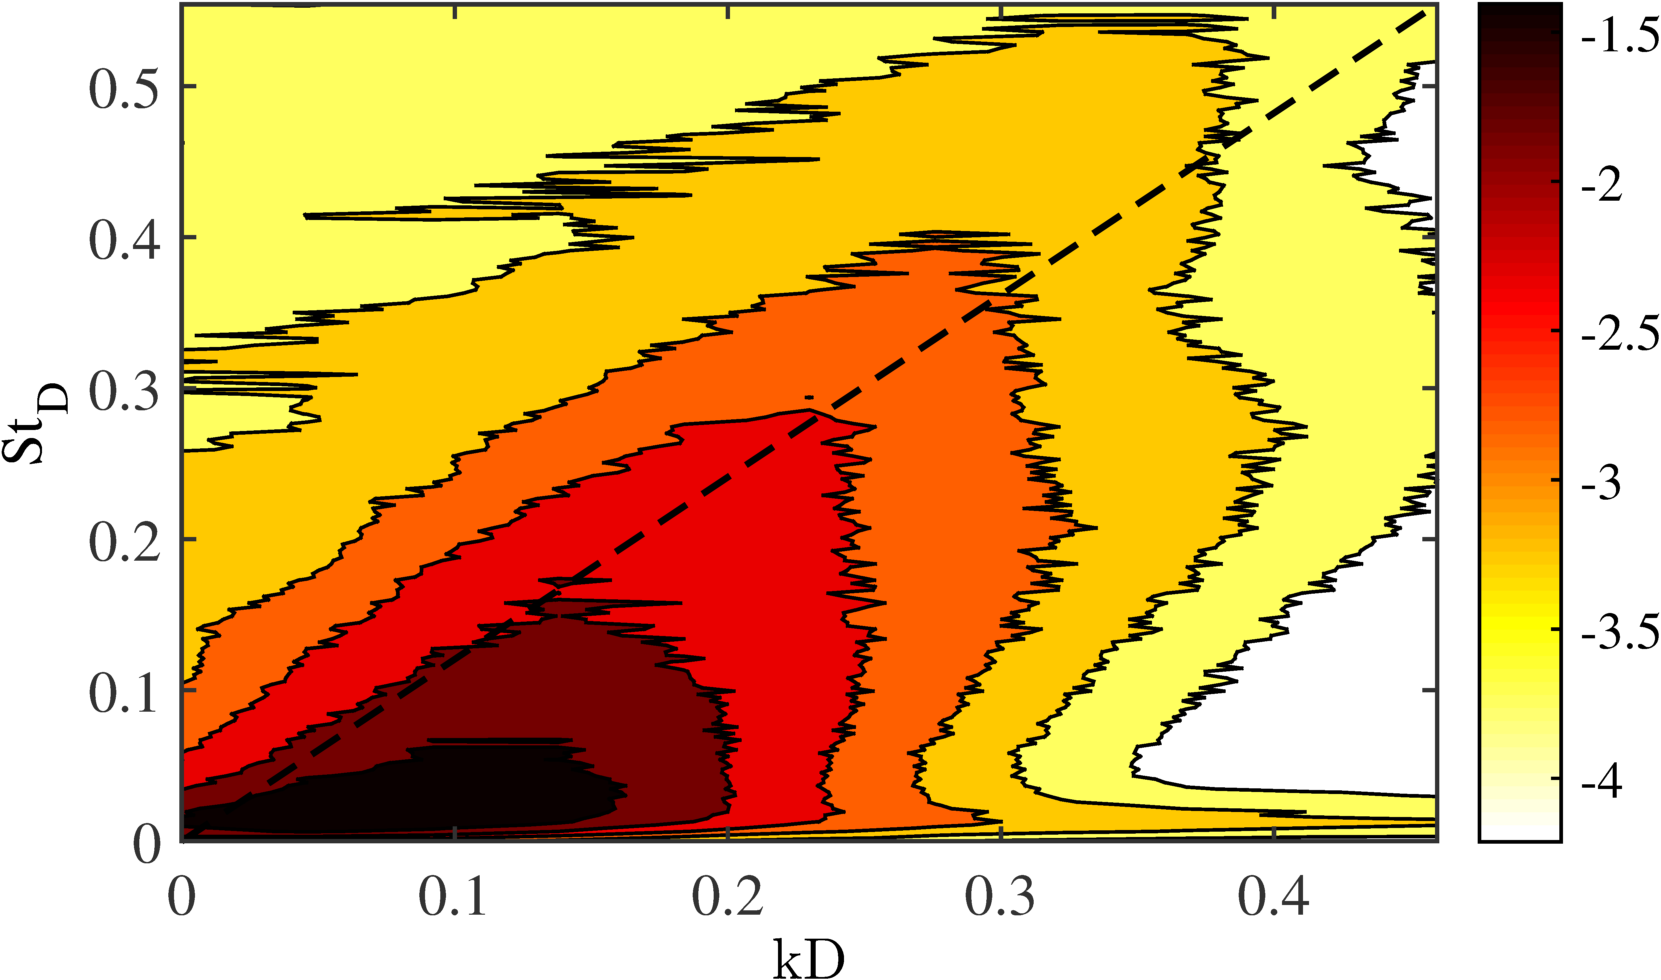
\includegraphics{Figures/Phase_Velocity_Map.png}
	\caption{Wavenumber-Frequency spectral energy.}
	\label{fig:phase_velocity_map}
\end{figure}

In the current work, the irrotational near-field pressure is decomposed into its constitutive hydrodynamic and acoustic components based on phase-velocity. 
The current method is similar to that of Tinney \& Jordan [cite] in that an axial array of many microphones is used, though it differs in how it identifies components of different phase-velocity.
Here, the filtering will be performed by a spatio-temporal continuous wavelet transform.

\subsection{The Wavelet Transform}
Fourier analysis is commonly employed in the aeroacoustics community to study fundamental aspects of jet noise due to its simplicity and the great abundance of information it can provide. 
However, there is also a great drawback associated with Fourier analysis: while it analyzes a given signal at a distinct frequency, local information for a given event is spread over all spectral coefficients. 
This is due to the fact that the basis functions used by the Fourier transform oscillate indefinitely. 
For a completely stationary signal this is not an issue, however it has become increasingly clear that the jet noise phenomenon is not a stationary process.
Transient events, such as intermittency or the spatial and temporal modulation of a wavepacket, have been shown to be important in the noise generation process. 

Grossman [cite] introduced the wavelet transform in an effort to overcome some of the shortcomings of the Fourier transform.
Unlike the Fourier transform, the wavelet transform involves a convolution of the signal with a set of basis functions which decay to zero at the bounds.
As a direct result, translation of the basis function in space and/or time is now meaningful. 
The basis functions (often referred to as the analyzing or daughter wavelets) are all derived from a single function, the mother wavelet, which must satisfy certain criteria [Farge],
Most notable of of these criteria is that of admissibility, which in essence requires that the wavelet must be of finite energy. 
In practice, it is also helpful to choose a mother wavelet which is well-localized in both the spatio-temporal domain and the frequency domain. 
For a given mother wavelet, $\psi (\vec{x})$, the daughter wavelets can be constructed as

\subsection{Validation}
\section{Identifying the Acoustic Source Region}